%追加すべき事項
\chapter{背景:音}

本章では、音の定義を行い、音の表現方法を紹介する。

\section{音の定義}

音とは、弾性体中を伝播する波により起こされる音波が聴覚により感じられるもののことである。

\subsection{音響信号}

音は時間方向の変化量であるため、音響信号と呼ばれる。音響信号は連続的な信号であるが、コンピュータで扱うために離散的な信号へと変換する必要がある。また、変換の際には標本化~(サンプリング)~と量子化が必要である。まず、サンプリングは一定の時間を空けて離散的に測定を行うことであり、1秒あたりのサンプリング回数をサンプリング周波数と呼ぶ。そして、量子化は信号の大きさを離散的に表現することであり、信号の大きさを表現するビット数を量子化ビット数と呼ぶ。

\subsection{楽音}

楽音は周期性のある音波を持つ音のことであり、音楽で用いられる。本論文では楽音としての音を生成することを目標とする。また、楽音は長さ、大きさ、高さ、音色の四要素を持つ。

\subsubsection{音の長さと大きさ}

音の長さは音波の時間長により決まり、音の大きさは音波の振幅により決まる~(\prettyref{fig:gakuon1})~。音波の時間長が長いほど音の長さは長くなり、音波の振幅が大きいほど音の大きさは大きい。

\subsubsection{音の高さと音色}

音の高さと音色は直感的にはそれぞれ音波の周期構造の長さと形により決まる~(\prettyref{fig:gakuon2})~。また、音の高さは音波の周波数により決まり、周波数の高い音ほど音の高さは高くなる。そして、音の長さと大きさと高さが同じ時の音の違いを音色と呼び、それぞれの楽器は異なる音色を持つ。

\begin{figure}[b]
\centering
\begin{minipage}{0.48\columnwidth}
\centering
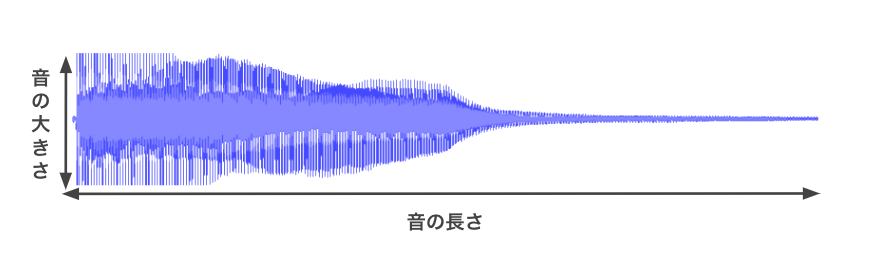
\includegraphics[width=\columnwidth]{figure/gakuon1.png}
\caption{音波}
\label{fig:gakuon1}
\end{minipage}
\begin{minipage}{0.48\columnwidth}
\centering
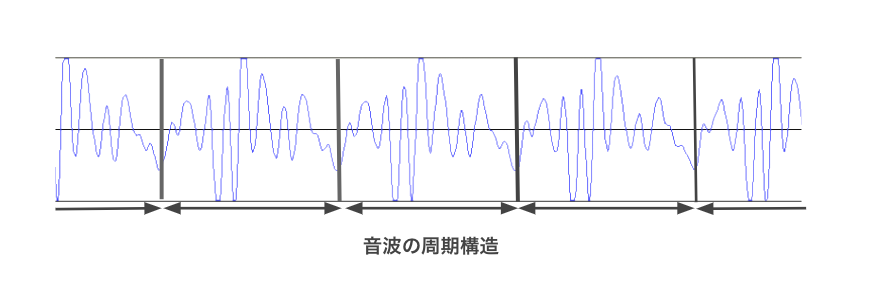
\includegraphics[width=\columnwidth]{figure/gakuon2.png}
\caption{音波の拡大図}
\label{fig:gakuon2}
\end{minipage}
\end{figure}

%ここで改ページ
\clearpage

\section{音の表現}

音をニューラルネットワークで扱うためには、楽音としての特徴を学習するための適切な表現を得る必要がある。また、本節は~\cite{musictutorial}の3.2節及び~\cite{timbretron}の2.1節を参考に作成し、本節の図は~\cite{musictutorial}のFigure~4と~\cite{timbretron}のFigure~2を利用している。

\subsection{一次元データと二次元データ}

音響信号をニューラルネットワークでは一次元データとして扱う~(\prettyref{fig:audio_signal})~。~\cite{Jukebox}や~\cite{WaveNet}ではこの一次元データをニューラルネットワークで扱うが、素朴な音の表現である一次元データから楽音としての特徴を学習するのは難しい。したがって、音響信号を周波数成分ごとに分解して二次元データに変換することが一般的である。また、二つの次元としては時間と周波数を選ぶことが多く、この場合の二次元データを時間-周波数表現と呼ぶ。

\subsection{STFT}

STFT~(Short~Time~Fourier~Transform)~は、時間-周波数表現の一般的な生成手法である。STFTでは中間周波数を利用した線形に等間隔のバンドパスフィルターを用いて音響信号を周波数成分ごとに分解する。また、STFTを用いて生成できる時間-周波数表現を可視化した画像をスペクトログラムと呼び、振幅の大きさを明度などにより表す~(\prettyref{fig:STFT})~。ただし、スペクトログラムには位相の情報は保持されないため、音響信号からスペクトログラムの変換は不可逆である。そして、離散信号に対してのSTFTは\prettyref{eq:STFT}により定式化される。また、$m$は時刻、$w_k$は周波数、$w$は0を中心とした窓関数、$x(n)$は時間$n$における信号$x$の値、である。

\begin{align}
    \label{eq:STFT}
    \operatorname{STFT}\left(m, \omega_k\right)=\sum_{n=-\infty}^{\infty} x(n) w(n-m) e^{-i \omega_k n}
\end{align}

また、人間の聴覚系の周波数分解能は線形からは遠く、STFTは楽音の解析のために作成されたものでもないため、スペクトログラムは周波数方向の圧縮のような工夫を施すことで用いられることが多い。

\begin{figure}[b]
\centering
\begin{minipage}[b]{0.48\columnwidth}
\centering
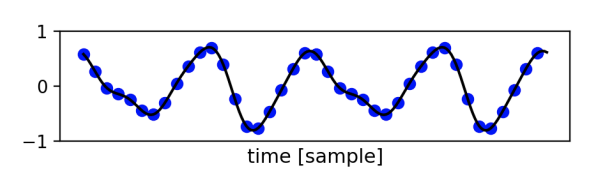
\includegraphics[width=\columnwidth]{figure/audio_signal.png}
\caption{音響信号}
\label{fig:audio_signal}
\end{minipage}
\begin{minipage}[b]{0.48\columnwidth}
\centering
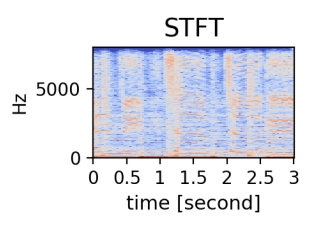
\includegraphics[width=\columnwidth]{figure/stft.png}
\caption{STFT}
\label{fig:STFT}
\end{minipage}
\end{figure}

%ここで改ページ
\clearpage

メルスペクトログラムは、周波数方向の圧縮の工夫を施したスペクトログラムとして一般的なものである~(\prettyref{fig:mel})~。メルスペクトログラムでは、人間の感じる音の高さの差と差が等しくなるように調整した尺度であるメル尺度~\cite{melscale}を用いて周波数方向の圧縮を行う。また、~\cite{mel}では周波数を$f$として\prettyref{eq:mel}のように定式化される。

\begin{align}
    \label{eq:mel}
    mel(f)=1127.01048\log{(\frac{f}{700}+1)}
\end{align}

メル尺度は人間の聴覚系に合わせた尺度であり、メルスペクトログラムはスペクトログラムよりも楽音の解析に適している。例えば、~\cite{GANSynth}では位相の情報を付加したメルスペクトログラムを用いて楽音の生成を行う。

\subsection{CQT}

CQT~(Constant~Q~Transform)~は音楽の解析のために主に二つの点でSTFTを改善した手法である。一つ目の改善点は、サンプル数についてである。STFTの場合は

CQT~(Constant~Q~Transform)~\cite{CQT}は対数振幅の中心周波数を使用した二次元の表現である。CQTは対数振幅を用いており、音の高さの分布に近い。詳しくは~\cite{CQT}を参考にされたい。

また、CQTにおいても\prettyref{fig:cqt}のようなスペクトログラムを生成することができる。この時、

\begin{figure}[b]
\centering
\begin{minipage}[b]{0.48\columnwidth}
\centering
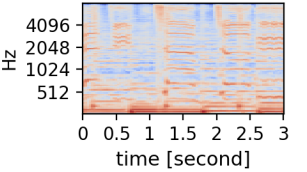
\includegraphics[width=\columnwidth]{figure/mel.png}
\caption{メルスペクトログラム}
\label{fig:mel}
\end{minipage}
\begin{minipage}[b]{0.48\columnwidth}
\centering
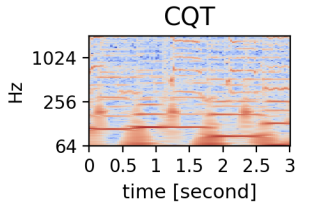
\includegraphics[width=\columnwidth]{figure/cqt.png}
\caption{CQT}
\label{fig:cqt}
\end{minipage}
\end{figure}
    